\label{sec:choiceOfMethod}
The main research question of this study was used to determine which research method would be the most fitting. The following is the question we arrived at:

\begin{itemize}
\item How do organizations perform information security incident management in practice?
\end{itemize}

Figure \ref{fig:methods} shows an overview of various research methods and three criteria that can be used to determine the appropriate research method for a study. The criteria are: form of research question, whether the study requires control of behavioural events and if the study focuses on contemporary events. The defined research question for this study is a so-called "how" question. The goal was to reveal current practices in organizations and the study did therefore not require control of any behavioural events. The study focuses mainly on contemporary events. Some past events such as incidents that have occurred are relevant, but the main focus is on current practices. Based on this, case study emerged as the most suitable method for this study, as shown in the figure.

There are other advantages to choosing case study as the research method for this study. Case studies can provide information that can help judge if specific technologies will benefit an organization or project \cite{kitchenham1995case}. This is applicable to our study and especially to the sub-question:

\begin{itemize}
\item To what extent are existing standards/guidelines adopted in plans for information security incident management?
\end{itemize}

This question seeks to identify if standards/guidelines are used and if they benefit an organization.

\begin{figure}[H]
\begin{center}
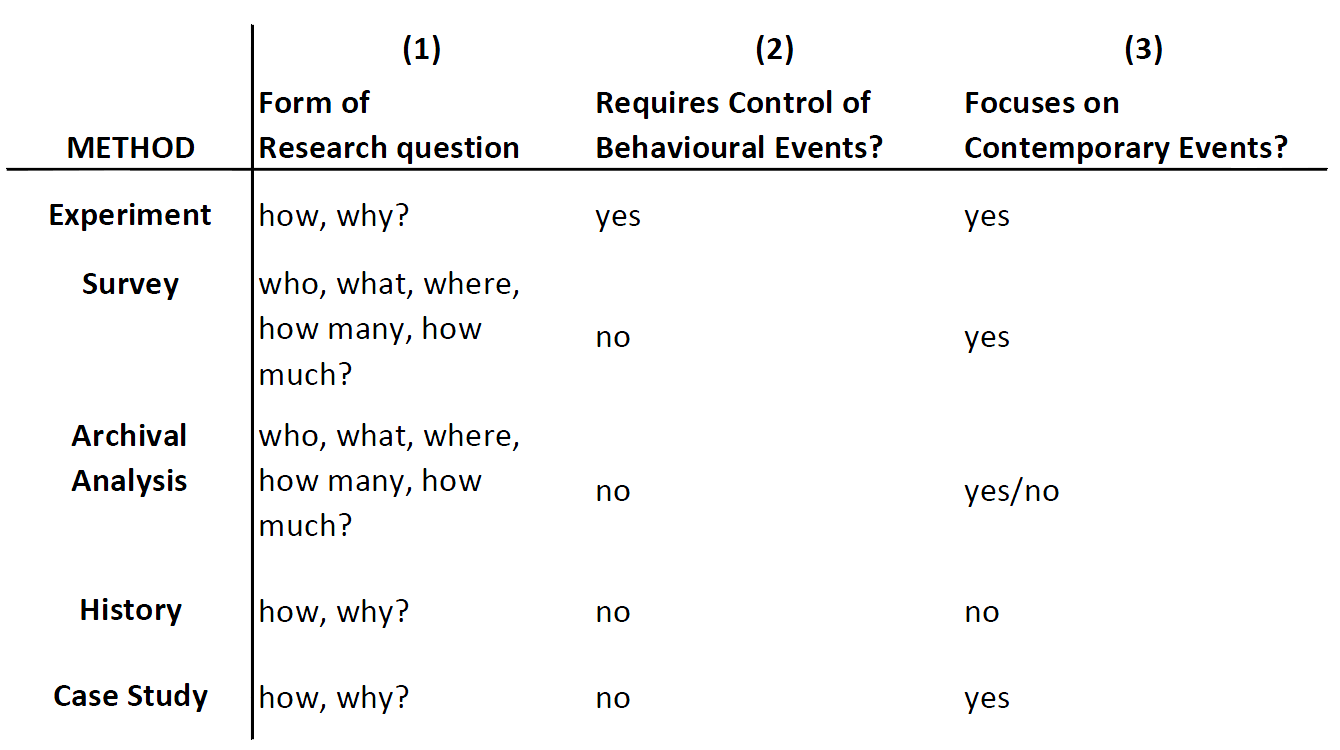
\includegraphics[scale=0.35]{methods.png}
\caption[Situations for different research methods]{Situations for different research methods, modified from \cite{CaseStudyResearch}}
\label{fig:methods}
\end{center}
\end{figure}

A case study is applicable to real-world projects, which is what we wanted to study. Another important advantage is that it can deal with various kinds of evidence, such as documents, archival records, interviews and artefacts.